\documentclass{beamer}
\usepackage[utf8]{inputenc}

\usetheme{Madrid}
\usecolortheme{default}
\usepackage{amsmath,amssymb,amsfonts,amsthm}
\usepackage{txfonts}
\usepackage{tkz-euclide}
\usepackage{listings}
\usepackage{adjustbox}
\usepackage{array}
\usepackage{tabularx}
\usepackage{gvv}
\usepackage{lmodern}
\usepackage{circuitikz}
\usepackage{tikz}
\usepackage{graphicx}
\usepackage{textcomp}
\usepackage{cancel}
\setbeamertemplate{page number in head/foot}[totalframenumber]

\usepackage{tcolorbox}
\tcbuselibrary{minted,breakable,xparse,skins}



\definecolor{bg}{gray}{0.95}
\DeclareTCBListing{mintedbox}{O{}m!O{}}{%
  breakable=true,
  listing engine=minted,
  listing only,
  minted language=#2,
  minted style=default,
  minted options={%
    linenos,
    gobble=0,
    breaklines=true,
    breakafter=,,
    fontsize=\small,
    numbersep=8pt,
    #1},
  boxsep=0pt,
  left skip=0pt,
  right skip=0pt,
  left=25pt,
  right=0pt,
  top=3pt,
  bottom=3pt,
  arc=5pt,
  leftrule=0pt,
  rightrule=0pt,
  bottomrule=2pt,
  toprule=2pt,
  colback=bg,
  colframe=orange!70,
  enhanced,
  overlay={%
    \begin{tcbclipinterior}
    \fill[orange!20!white] (frame.south west) rectangle ([xshift=20pt]frame.north west);
    \end{tcbclipinterior}},
  #3,
}
\lstset{
    language=C,
    basicstyle=\ttfamily\small,
    keywordstyle=\color{blue},
    stringstyle=\color{orange},
    commentstyle=\color{green!60!black},
    numbers=left,
    numberstyle=\tiny\color{gray},
    breaklines=true,
    showstringspaces=false,
}
%------------------------------------------------------------
%This block of code defines the information to appear in the
%Title page
\title %optional
{5.9.3}
\date{}
%\subtitle{A short story}

\author % (optional)
{Sai Krishna Bakki - EE25BTECH11049}

\begin{document}
\frame{\titlepage}
\begin{frame}{Question}
Two schools \textbf{P} and \textbf{Q} decided to award prizes to their students for two games of Hockey \rupee~x per students and cricket \rupee~y per student. School \textbf{P} decided to award a total of \rupee~9,500 for the two games to 5 and 4 students respectively; while school \textbf{Q} decided to award \rupee~7,370 for the two games to 4 and 3 students respectively. Based on the given information, answer the following questions :
\begin{enumerate}
    \item Represent the following information algebraically (in terms of x and y).
    \item \begin{enumerate}
        \item What is the prize amount for hockey ?
        \item Prize amount on which game is more and by how much ?
    \end{enumerate}
    \item What will be the total prize amount if there are 2 students each from two games ?
\end{enumerate}
\end{frame}
\begin{frame}{Theoretical Solution}
    Given\\
For Schools \textbf{P} and \textbf{Q}:\\
\begin{align}
5x + 4y = 9500 \\
4x + 3y=7370\\
\implies
\myvec{5&4\\4&3}\myvec{x\\y}=\myvec{9500\\7370}
\end{align}
\begin{align}
    \augvec{2}{1}{5&4&9500\\4&3&7370}\xleftrightarrow{R_1\rightarrow R_1-R_2}\augvec{2}{1}{1&1&2130\\4&3&7370}\\
    \augvec{2}{1}{1&1&2130\\4&3&7370}\xleftrightarrow{R_2\rightarrow R_2-4R_2}\augvec{2}{1}{1&1&2130\\0&-1&-1150}\\
    \augvec{2}{1}{1&1&2130\\0&-1&-1150}\xleftrightarrow{R_1\rightarrow R_1+R_2}\augvec{2}{1}{1&0&980\\0&-1&-1150}
    \end{align}
\end{frame}
\begin{frame}{Theoretical Solution}
\begin{align}
    \augvec{2}{1}{1&0&980\\0&-1&-1150}\xleftrightarrow{R_2\rightarrow -R_2}\augvec{2}{1}{1&0&980\\0&1&1150}\\
    \myvec{x\\y}=\myvec{980\\1150}
\end{align}
$\therefore$ The prize amount for Hockey(x) and Cricket(y) respectively are \rupee~980 and \rupee~1150.
The Prize amount of Cricket is more than Hockey by a difference of \rupee~170.
\begin{align}
    \text{Total amount}= \myvec{2&2}\myvec{x\\y}\\
    \text{Total amount}= \myvec{2&2}\myvec{980\\1150}\\
    \text{Total amount}=1960+2300 \notag\\
    =4260
\end{align}
$\therefore$ The total prize amount if there are 2 students each from two games is \rupee~4260.
\end{frame}
\begin{frame}[fragile]
\frametitle{C Code}
\begin{lstlisting}
#include <stdio.h>
#include <math.h> // Required for fabs()

// This function solves a system of two linear equations using an augmented matrix
// and Gaussian elimination.
// a*x + b*y = e
// c*x + d*y = f
void solve_system(double a, double b, double c, double d, double e, double f, double* x, double* y) {
    // Create the augmented matrix: [ a b | e ]
    //                               [ c d | f ]
    double aug_matrix[2][3] = {
        {a, b, e},
        {c, d, f}
    };
\end{lstlisting}
\end{frame}
\begin{frame}[fragile]
\frametitle{C Code}
\begin{lstlisting}
    // --- Forward Elimination to get Row-Echelon Form ---

    // If the pivot (a) is zero, swap the rows to avoid division by zero.
    if (fabs(aug_matrix[0][0]) < 1e-9) {
        for (int i = 0; i < 3; i++) {
            double temp = aug_matrix[0][i];
            aug_matrix[0][i] = aug_matrix[1][i];
            aug_matrix[1][i] = temp;
        }
    }

    // Check if the pivot is still zero, which means no unique solution exists.
    if (fabs(aug_matrix[0][0]) < 1e-9) {
        *x = -1.0/0.0; // Represents NaN
        *y = -1.0/0.0; // Represents NaN
        return;
    }
\end{lstlisting}
\end{frame}
\begin{frame}[fragile]
\frametitle{C Code}
\begin{lstlisting}
    // Perform the row operation: R2 -> R2 - (c/a) * R1
    double factor = aug_matrix[1][0] / aug_matrix[0][0];
    aug_matrix[1][0] = 0.0; // This is the goal
    aug_matrix[1][1] -= factor * aug_matrix[0][1];
    aug_matrix[1][2] -= factor * aug_matrix[0][2];

    // --- Back Substitution ---

    // Check if the second pivot element is zero. If so, there's no unique solution.
    if (fabs(aug_matrix[1][1]) < 1e-9) {
        *x = -1.0/0.0; // NaN
        *y = -1.0/0.0; // NaN
        return;
    }
\end{lstlisting}
\end{frame}
\begin{frame}[fragile]
\frametitle{C Code}
\begin{lstlisting}
    // Solve for y from the second row: (d')*y = f'
    *y = aug_matrix[1][2] / aug_matrix[1][1];

    // Solve for x from the first row: a*x + b*y = e  => x = (e - b*y) / a
    *x = (aug_matrix[0][2] - aug_matrix[0][1] * (*y)) / aug_matrix[0][0];
}
\end{lstlisting}
\end{frame}
\begin{frame}[fragile]
\frametitle{Python Through Shared Output}
\begin{lstlisting}
import ctypes
import numpy as np
import matplotlib.pyplot as plt
from libs.funcs import line_dir_pt, param_norm

# --- Ctypes setup to call the C function ---

# Load the shared library.
# NOTE: You must compile the corresponding C file into a shared library first.
# On Linux/macOS, use: gcc -shared -o intersection.so -fPIC your_c_file.c
try:
    # The script was named intersection.py, so we assume the shared library
    # might be named intersection.so
    solver_lib = ctypes.CDLL('./line.so')
except OSError:
\end{lstlisting}
\end{frame}
\begin{frame}[fragile]
\frametitle{Python Through Shared Output}
\begin{lstlisting}
print("Error: Could not find 'line.so'.")
print("Please ensure the C code is compiled into a shared library named 'line.so'.")
exit()

# Define the function signature from the C code.
solve_system_c = solver_lib.solve_system
solve_system_c.argtypes = [ctypes.c_double, ctypes.c_double, ctypes.c_double, ctypes.c_double, ctypes.c_double, ctypes.c_double, ctypes.POINTER(ctypes.c_double), ctypes.POINTER(ctypes.c_double)]
solve_system_c.restype = None
# --- Solving the system of equations ---

# The first equation is 5x + 4y = 9500
a, b, e = 5.0, 4.0, 9500.0

# The second equation is 4x + 3y = 7370
c, d, f = 4.0, 3.0, 7370.0
\end{lstlisting}
\end{frame}
\begin{frame}[fragile]
\frametitle{Python Through Shared Output}
\begin{lstlisting}
# Create pointers for the output variables x and y
x = ctypes.c_double()
y = ctypes.c_double()

# Call the C function to solve the system
solve_system_c(a, b, c, d, e, f, ctypes.byref(x), ctypes.byref(y))

# Get the Python values from the ctypes objects
x_sol, y_sol = x.value, y.value

print(f"The solution from the C library is:")
print(f"x = {x_sol}")
print(f"y = {y_sol}")

# --- Verification and Plotting ---
print("\nVerification:")
# Note: Due to floating-point precision, the result might be extremely close but not exactly the integer value.
\end{lstlisting}
\end{frame}
\begin{frame}[fragile]
\frametitle{Python Through Shared Output}
\begin{lstlisting}
print(f"5*({x_sol}) + 4*({y_sol}) = {5*x_sol + 4*y_sol}")
print(f"4*({x_sol}) + 3*({y_sol}) = {4*x_sol + 3*y_sol}")

# Normal vectors for plotting
n1 = np.array([[a], [b]])
c1 = e
n2 = np.array([[c], [d]])
c2 = f

# Generate points for the first line (widened range for visibility)
m1, A1 = param_norm(n1, c1)
line1_pts = line_dir_pt(m1, A1, -5000, 5000)

# Generate points for the second line (widened range for visibility)
m2, A2 = param_norm(n2, c2)
line2_pts = line_dir_pt(m2, A2, -5000, 5000)
\end{lstlisting}
\end{frame}
\begin{frame}[fragile]
\frametitle{Python Through Shared Output}
\begin{lstlisting}
# Plot the lines
plt.plot(line1_pts[0,:], line1_pts[1,:], label='5x + 4y = 9500')
plt.plot(line2_pts[0,:], line2_pts[1,:], label='4x + 3y = 7370')
# Plot the intersection point
plt.plot(x_sol, y_sol, 'o', markersize=8, label=f'Intersection ({x_sol:.2f}, {y_sol:.2f})')
# Draw x and y axes
plt.axhline(0, color='black', linewidth=0.5)
plt.axvline(0, color='black', linewidth=0.5)

# Add labels and title for clarity
plt.xlabel("x-axis")
plt.ylabel("y-axis")
plt.title("Intersection of Two Lines (Solved with C)")
plt.grid(True)
plt.legend()
plt.axis('equal')
plt.show()
\end{lstlisting}
\end{frame}
\begin{frame}[fragile]
\frametitle{Python Code}
\begin{lstlisting}
import numpy as np
from libs.funcs import line_isect, line_dir_pt, param_norm
import matplotlib.pyplot as plt

# The first equation is 5x + 4y = 9500
# The normal vector n1 is the coefficients of x and y
n1 = np.array([[5], [4]])
# The constant c1 is 9500
c1 = 9500

# The second equation is 4x + 3y = 7370
# The normal vector n2 is the coefficients of x and y
n2 = np.array([[4], [3]])
# The constant c2 is 7370
c2 = 7370

# The line_intersect function from funcs.py solves the system of equations.
\end{lstlisting}
\end{frame}
\begin{frame}[fragile]
\frametitle{Python Code}
\begin{lstlisting}
# It takes the two normal vectors and two constants as input.
# The system can be represented as:
# [5 4] [x] = [9500]
# [4 3] [y]   [7370]
solution = line_isect(n1, c1, n2, c2)

print(f"The solution to the system of equations is:")
print(f"x = {solution[0][0]}")
print(f"y = {solution[1][0]}")

# Verification
# Let's plug the values back into the equations to check
x = solution[0][0]
y = solution[1][0]

print("\nVerification:")
# Note: Due to floating-point precision, the result might be extremely close but not exactly the integer value.
\end{lstlisting}
\end{frame}
\begin{frame}[fragile]
\frametitle{Python Code}
\begin{lstlisting}
print(f"5*({x}) + 4*({y}) = {5*x + 4*y}")
print(f"4*({x}) + 3*({y}) = {4*x + 3*y}")

# Plotting the lines and the intersection point
# Generate points for the first line (widened range for visibility)
m1, A1 = param_norm(n1, c1)
line1_pts = line_dir_pt(m1, A1, -5000, 5000)

# Generate points for the second line (widened range for visibility)
m2, A2 = param_norm(n2, c2)
line2_pts = line_dir_pt(m2, A2, -5000, 5000)

# Plot the lines
plt.plot(line1_pts[0,:], line1_pts[1,:], label='5x + 4y = 9500')
plt.plot(line2_pts[0,:], line2_pts[1,:], label='4x + 3y = 7370')
\end{lstlisting}
\end{frame}
\begin{frame}[fragile]
\frametitle{Python Code}
\begin{lstlisting}
# Plot the intersection point
plt.plot(solution[0], solution[1], 'o', markersize=8, label=f'Intersection ({x:.2f}, {y:.2f})')

# Draw x and y axes
plt.axhline(0, color='black', linewidth=0.9)
plt.axvline(0, color='black', linewidth=0.9)

# Add labels and title for clarity
plt.xlabel("x-axis")
plt.ylabel("y-axis")
plt.title("Intersection of Two Lines")
plt.grid(True)
plt.legend()
plt.axis('equal') # Ensures the axes are scaled equally
plt.show()
\end{lstlisting}
\end{frame}
\begin{frame}{Plot By C code and Python Code}
    \begin{figure}
    \centering
    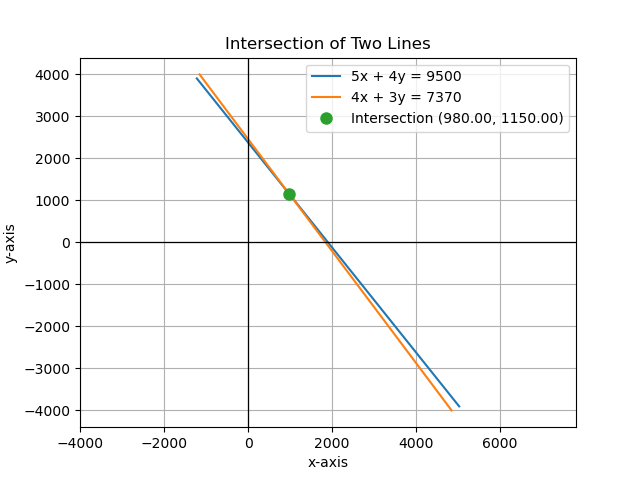
\includegraphics[width=0.7\columnwidth]{figs/Figure_1.png}
    \label{fig:placeholder}
    \caption{1}
\end{figure}
\end{frame}
\end{document}